%!TEX root = ../../tcc.tex

\subsection*{Kademlia}

O Kademlia é um \gls*{dht} criado em 2002 \cite{artigo:kademlia} com o objetivo de
melhorar os métodos de busca atuais (Napster e \gls*{gnutella}), que eram ineficientes.
Assim como os outros algoritmos de \gls*{dht}, ele se baseou na estrutura informalmente
conhecida como \enquote{rede de Plaxton} (\emph{Plaxton mesh}), nome que remete a um
dos seus autores \cite{artigo:dht}. Por ter causado boas impressões, foi usado na
implementação da busca de arquivos no programa cliente eMule.

O algoritmo implementa uma rede \emph{overlay} cuja estrutura e comunicação se baseiam
na procura de seus nós. Cada um destes nós é identificado por um identificador único
(ID), que serve tanto para a identificação quanto para a localização de valores na
\gls*{hashtable}.

Outro ponto é que todos os nós são tratados como folhas de uma árvore binária, cujas
posições são estabelecidas pelo menor prefixo comum de seus IDs, e organizando-os de
forma que, para um dado nó $x$, a árvore é dividida em várias subárvores menores que
não o contém. Assim, a maior subárvore consiste de metade da árvore que não contém $x$,
a subárvore seguinte é feita da metade da árvore restante onde $x$ também não está
contido, etc. O Kademlia garante ainda que todo nó conhece um outro que está em cada
uma das subárvores, se estas contiverem algum nó.

\begin{figure}[ht!]
    \centering
    \fbox{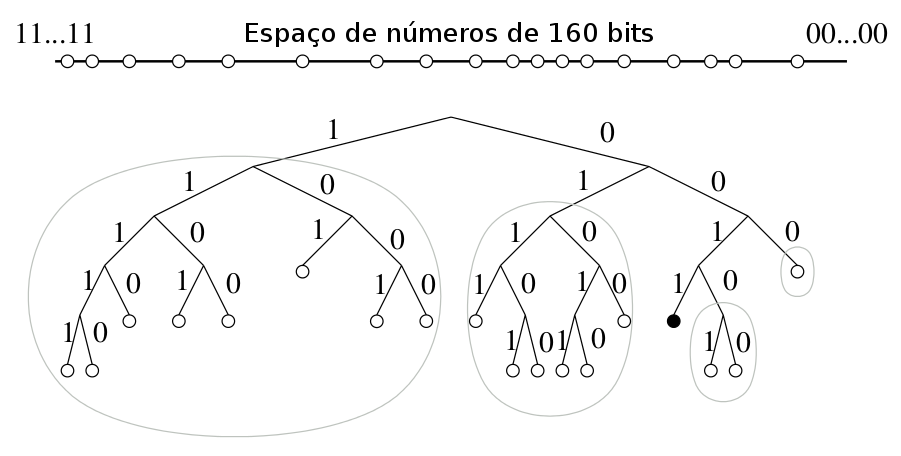
\includegraphics[width=\textwidth]{dht1.png}}
    \caption{Árvore binária do Kademlia. O nó preto é a posição do ID 0011...; os ovais
    cinzas são as subárvores onde o nó preto deve possuir nós conhecidos. Fonte:
    \cite{artigo:kademlia}}
    \label{fig:dht-arvore}
\end{figure}

Durante uma busca, o processo deve conhecer a chave (que é um
\gls*{hashvalue}) associado ao objeto - neste caso, o ID do \gls*{torrent}, que é seu
\gls*{hashvalue} - e explora a rede em passos, encontrando nós mais próximos da chave,
até encontrar o valor buscado ou não nós existirem mais próximos que o atual. Dessa
forma, para uma rede com $n$ nós, o algoritmo visita apenas $O(\log n)$ nós.

\begin{figure}[ht!]
    \centering
    \fbox{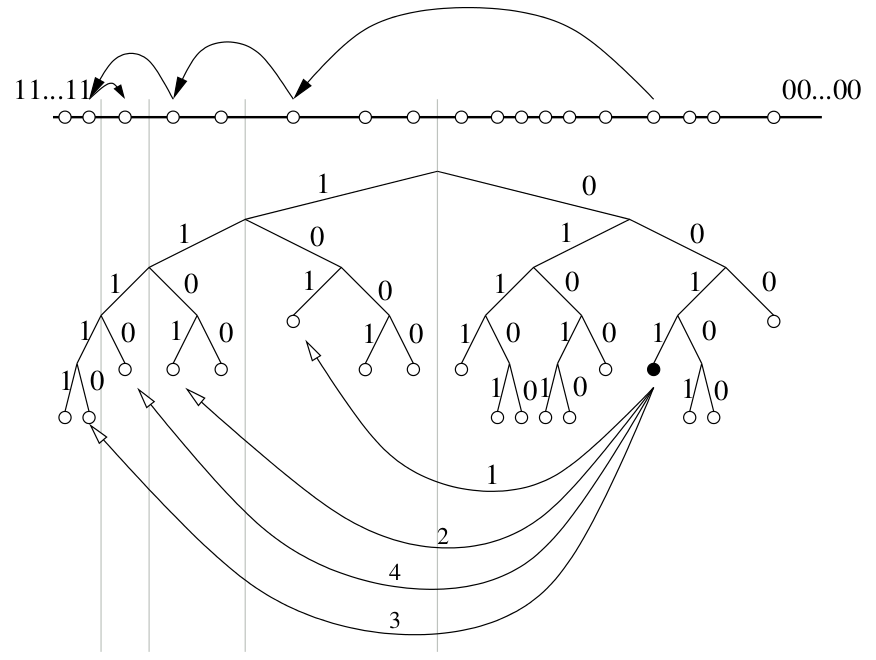
\includegraphics[width=\textwidth]{dht2.png}}
    \caption{Exemplo de uma busca na árvore de nós do Kademlia usando-se um ID. O nó
    preto, de prefixo 0011, encontra o nó de prefixo 1110 através de sucessivas buscas
    (setas numeradas inferiores). As setas superiores mostram a convergência da
    busca durante a execução. Fonte: \cite{artigo:kademlia}}
    \label{fig:dht-arvore-busca}
\end{figure}